%%%%%%%%%%%%%%%%%%%%%%%%%%%%%%%%%%%%%%%%%%%%%%%%%%
%%%%%%%%%%
% Figures

\newpage

\section{Figures}

% Figure 1
\begin{figure}[htbp]
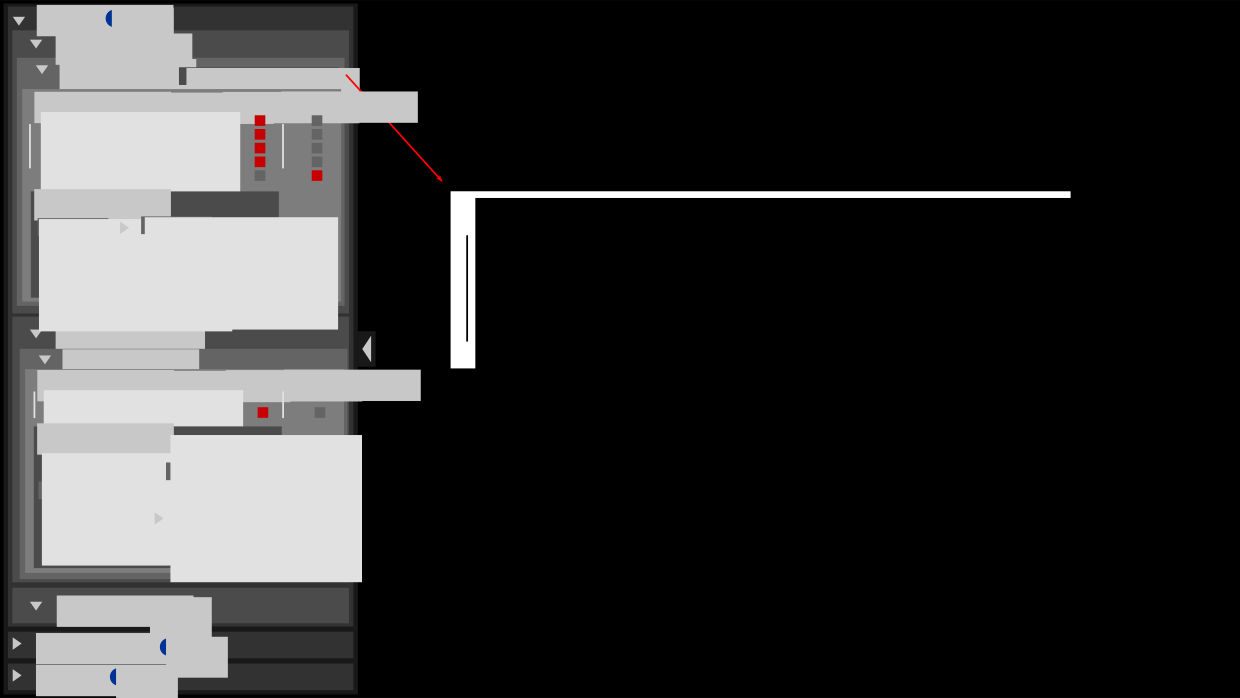
\includegraphics[scale=0.5]{sketch_2017-01-02_1}
\centering
\caption{This figure illustrates the \textbf{Query Interface} with lists of entities and properties for use in the query. It also shows an example of a table of entities along with custom properties, such as additional biological properties or experimental attributes, that the user can load from file.}
\label{fig:2017-01-02_1}
\end{figure}

% Figure 2
\begin{figure}[htbp]
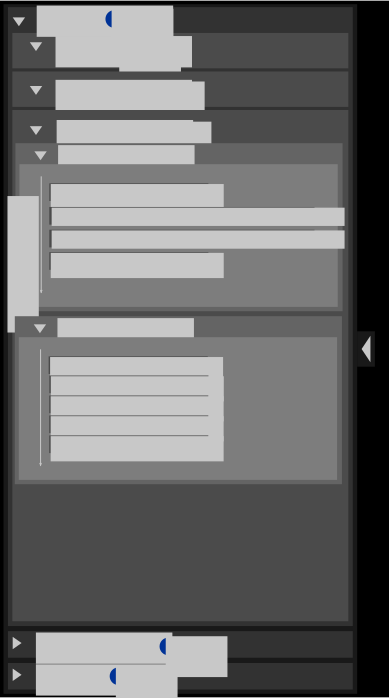
\includegraphics[scale=1]{sketch_2017-01-02_2}
\centering
\caption{This figure illustrates the \textbf{Query Interface} with sections to control the execution sequence of the query and to display results from the query.}
\label{fig:2017-01-02_2}
\end{figure}

% Figure 3
\begin{figure}[htbp]
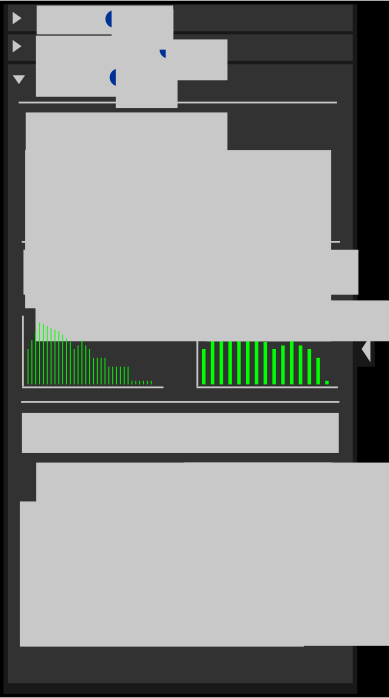
\includegraphics[scale=1]{sketch_2017-01-02_3}
\centering
\caption{This figure illustrates the \textbf{Detail Interface} with charts depicting the distribution of metabolite degrees and betweenness centralities and the distribution of metabolites between cellular compartments.}
\label{fig:2017-01-02_3}
\end{figure}

% Figure 4
\begin{figure}[htbp]
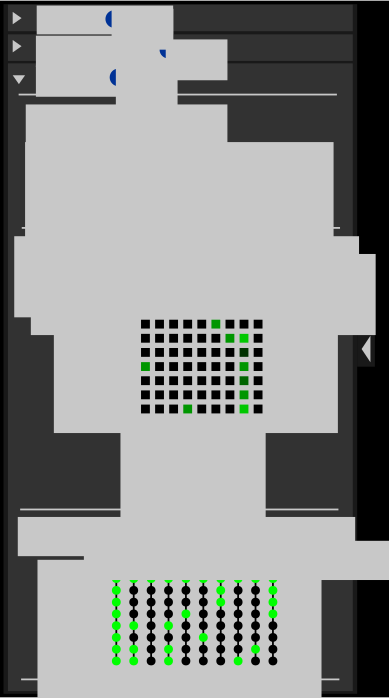
\includegraphics[scale=1]{sketch_2017-01-02_4}
\centering
\caption{This figure illustrates the \textbf{Detail Interface} with charts depicting the count of transport events between cellular compartments and the distribution of shared metabolites between combinations of multiple compartments.}
\label{fig:2017-01-02_4}
\end{figure}

% Figure 5
\begin{figure}[htbp]
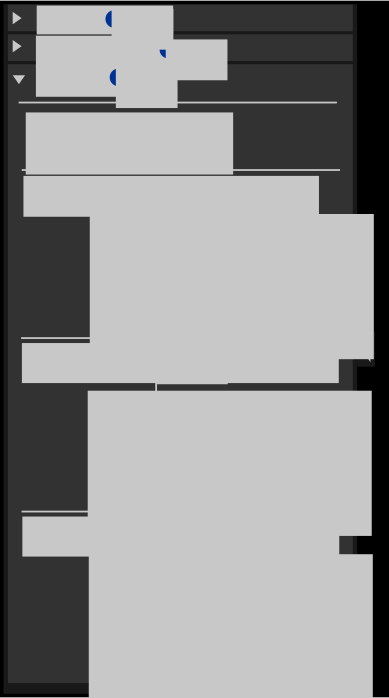
\includegraphics[scale=1]{sketch_2017-01-02_5}
\centering
\caption{This figure illustrates the \textbf{Detail Interface} with information in detail for a single metabolite.}
\label{fig:2017-01-02_5}
\end{figure}

% Figure 6
\begin{figure}[htbp]
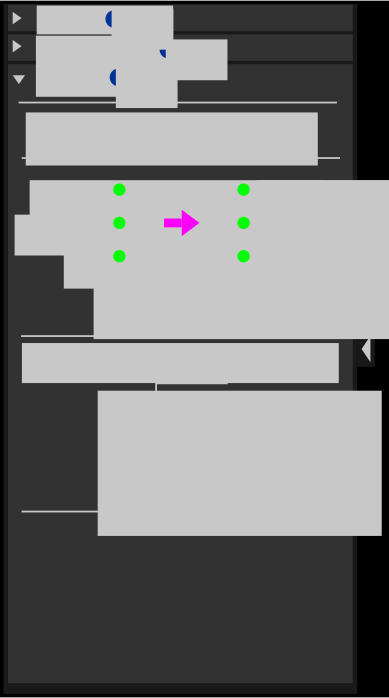
\includegraphics[scale=1]{sketch_2017-01-02_6}
\centering
\caption{This figure illustrates the \textbf{Detail Interface} with information in detail for a single reaction.}
\label{fig:2017-01-02_6}
\end{figure}

% Figure 7
\begin{figure}[htbp]
\includegraphics[scale=0.5]{sketch_2017-01-02_7}
\centering
\caption{This figure illustrates the \textbf{Navigation Interface} and the \textbf{Exploration Interface} without representation of properties by either position or color.}
\label{fig:2017-01-02_7}
\end{figure}

% Figure 8
\begin{figure}[htbp]
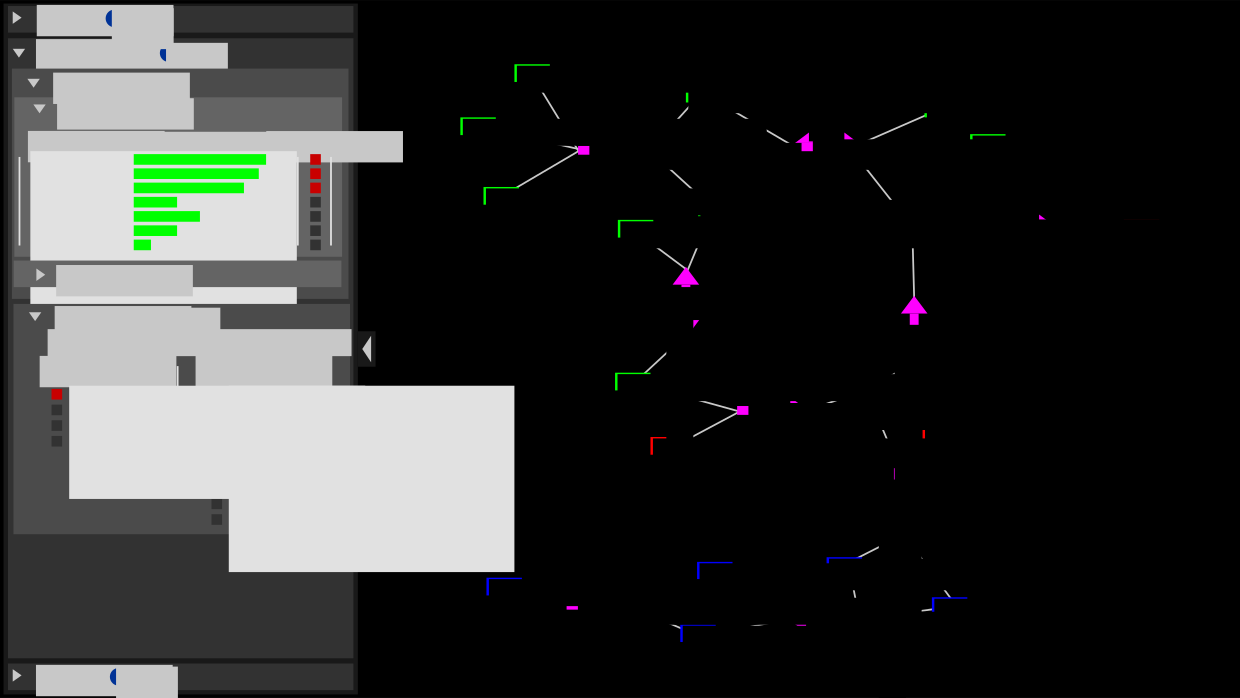
\includegraphics[scale=0.5]{sketch_2017-01-02_8}
\centering
\caption{This figure illustrates the \textbf{Navigation Interface} and the \textbf{Exploration Interface} with representation of pathway in color.}
\label{fig:2017-01-02_8}
\end{figure}

% Figure 9
\begin{figure}[htbp]
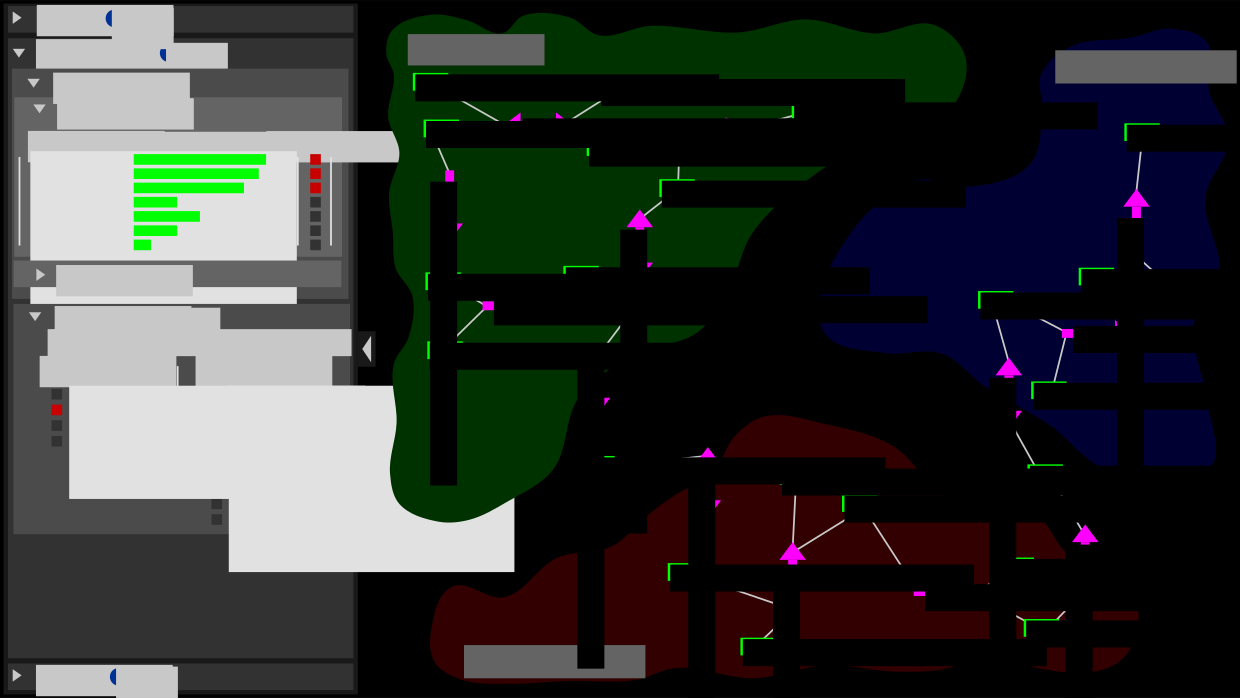
\includegraphics[scale=0.5]{sketch_2017-01-02_9}
\centering
\caption{This figure illustrates the the \textbf{Navigation Interface} and the \textbf{Exploration Interface} with representation of cellular compartment by position.}
\label{fig:2017-01-02_9}
\end{figure}

% Figure 10
\begin{figure}[htbp]
\includegraphics[scale=0.5]{sketch_2017-01-02_10}
\centering
\caption{This figure illustrates the \textbf{Navigation Interface} and the \textbf{Exploration Interface} with representation of cellular compartment by position and fold change by color.}
\label{fig:2017-01-02_10}
\end{figure}
